%%
% TUM Corporate Design LaTeX Templates
% Based on the templates from https://www.tum.de/cd
%
% Feel free to join development on
% https://gitlab.lrz.de/tum-templates/templates
% and/or to create an issue in case of trouble.
%
% tum-article class for scientific articles, reports, exercise sheets, ...
%
%%

\documentclass[twocolumn]{tum-article}
%\documentclass[twocolumn, german]{tum-article}
%\documentclass[times, twocolumn]{tum-article}
%\documentclass[times]{tum-article}
%\documentclass{tum-article}

%\usepackage{lipsum}

\title{Analysis of the 2014 Passenger Flight Network}
\author{Felix Paul Niemeyer\authormark{1},
	Saicharan Kumar\authormark{2}}
% Author 3\authormark{1}\orcid{0000-0000-0000-0000}}

% if too long for running head
\titlerunning{TUM Article}
\authorrunning{Author 1 et al.}

%\email{niemeyer.felix@tum.de}

\affil[1]{felix.niemeyer@tum.de, MiM}
\affil[2]{saicharan.kumar@tum.de, MiM}

\date{Received: 19.02.2020 - This is work in progress}

\begin{document}

\maketitle

\begin{abstract}
	In this case study we are looking at a dataset about air travel in 2014. We implement some mechanisms to clean the data, as well as mechanisms to enrich this dataset with information we query from wikidata. We estimate some missing data. Starting from there, we analyze some network characteristics for the whole network as well as airline-specific sub-networks. We compare airline-specific networks and find relations between their network's characteristics and their business model. We propose one metric that plays a role in forcasting whether a cooperation between two airlines is advantageous and use this metric to generate an alliances landscape. We compare it's predictive correctness to the real world by looking at the formation of Vanilla Airlines which occured in the year after the one our data stems from. 
\end{abstract}

\section{Data Description}
The network analysis is based on dataset from openflights.org. 
It describes passenger flight connections between airports in the year 2014. 
The data includes, which airline each connection is operated by.
The data comes in three tables: airports, routes and airlines. 
The airports table has entries for every airport with the following useful information: \\
- airport id\\
- iata and icao codes\\
- geographic coordinates\\
- country and region\\

The routes table lists an entrie for each connection between two airports that was operated by an airline somewhen in the year 2014. It does not contain any information about flight frequencies or passenger volume. The airline table lists airlines associated with their name and some information we do not need like country or callsign. \\

We are loading these files into an sqlite database for easier handling. 
We apply some queries for cleaning the data, e.g. removing routes operated by unknown airlines or filling in airport ids in routes where only iata or icao code is used to refer to a source or destination airport. \\

All the data-setup can be acomplished by running a single script.
This script and also all other code we have written for this project can be found in a public repository \cite{repository}.

\section{Data Enrichment \& Estimation}
After cleaning up the data, there are 3139 airports. 
Interpreting the data as a graph gives us a multiedge directed graph).
Looking at the degree distribution in Figure~\ref{fig:degree_distribution}, the alternating characteristic of degrees strikes the eye. It comes from the fact, that it's very uncommon for a connection between airports to exist only in one direction. Thus, there is much fewer nodes with odd degrees than than with even degrees. 

When we disregard odd degress, the seemingly linear distribution on a log log scale becomes apparent. Using least square (scipy.optimize.curve\_fit), we optimize paramters $c$ and $\gamma$ Figure~\ref{fig:degree_distribution_curves}

\begin{figure}
	\centering
	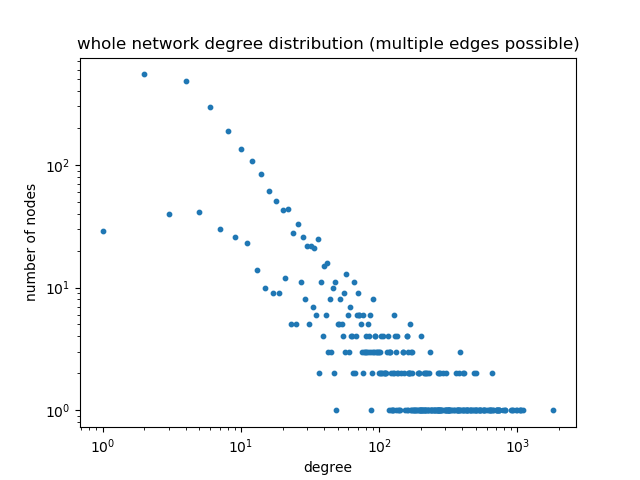
\includegraphics[width=76mm]{imgs/results/degree_distribution_incl_odd_degrees.png}
	\caption{
The degree distribution of the network on a log log scale }
	\label{fig:degree_distribution}
\end{figure}

\begin{figure}
	\centering
	\includegraphics[width=76mm]{imgs/results/degree_distribution_curve_manual.png}
	\caption{
Looking at even degrees only. Trying least square curve fitting to find suitable parameters for power law distribution function $f(x) = a * x^{-\gamma}$}
	\label{fig:degree_distribution_curves}
\end{figure}

Besides the main subgraph, that includes 3113 nodes, there are 6 small disconnected ones with only a couple of nodes.
One with 10 nodes for example Figure~\ref{fig:new_caledonia}, consists only of airports that are located in New Caledonia, an archipelago in the Pacific Ocean. 
\begin{figure}
	\centering
	\includegraphics[width=76mm]{imgs/new-caledonia-subgraph.png}
	\caption{Airports of New Caledonia drawn on a map}
	\label{fig:new_caledonia}
\end{figure}

In order to enable us to do more meaningful analysis, we enrich the dataset with additional information. We chose the airport patronage and found out, that we can get this data from Wikidata. 
For 1956 of the 3139 airports from the dataset, we can find patronage data from Wikidata. 
<describe how we do it: yearly vs. monthly + scaling from other years>
In order to populate the remaining nodes with reasonable patronages as well, we tried different techniques. 
First <using available data: runways -> factor -> calc. patronage per square feet + threshold, bad data quality. Show flow estimation iteration.>
Seccond <inspired by professor: algorithm that looks at neighboring airports patronage. Describe Algorithm. Show flow estimation iteration>

After estimating missing patronage data by looking at neighboring airports patronages, 14 airports without patronage remain. These must be in airports in disconnected subgraphs, because the algorithm would eventually reach them and assign a patronage otherwise. Investigations confirm that. We disregard these few dataless airports from disconnected subgraphs in the following analysises and thus end up with a network of 3125 airports. 

<Passenger flow estimation algorithm, outcomes>

\section{Basic Network Analysis}


\section{Airline Subnetwork Analysis \& Comparison}


\section{Airline Cooperation Opportunity}

The possibility to provide convenient on-line connections to clients is an important factor that drives welfare gains through ailine cooperation according to E. E. Bailey and D. Liu \cite{airline_consolidation_and_consumer_welfare}.

\section{Reality Check: Vanilla Airlines}


\section*{Acknowledgements}


\bibliographystyle{IEEEtran}
\bibliography{literature}

\end{document}
